\documentclass[tikz,border=8pt]{standalone}
% Shared look for every TikZ diagram. Load with \input{../../tools/tikz-style.tex}
\usepackage[T1]{fontenc}
\usepackage{lmodern}
\renewcommand{\sfdefault}{lmr}  % diagrams use the same serif as the text
\usetikzlibrary{arrows.meta, positioning, shapes.geometric, calc, fit, backgrounds}
\definecolor{cblue}{HTML}{4C78A8}
\definecolor{corange}{HTML}{F58518}
\definecolor{cgreen}{HTML}{54A24B}
\definecolor{cred}{HTML}{E45756}
\definecolor{cpurple}{HTML}{B279A2}
\definecolor{cgrey}{HTML}{6B6B6B}
\tikzset{
  every picture/.style={font=\sffamily, line width=1.2pt},
  box/.style={draw=#1, fill=#1!12, rounded corners=4pt, align=center, inner sep=7pt, minimum height=1.1cm},
  box/.default=cgrey,
  arrow/.style={-{Stealth[length=3mm]}, draw=cgrey, line width=1.4pt},
  title/.style={font=\sffamily\bfseries\Large},
  note/.style={font=\sffamily\small, text=cgrey, align=center},
}
\AtBeginDocument{\hyphenpenalty=10000 \exhyphenpenalty=10000}

\begin{document}
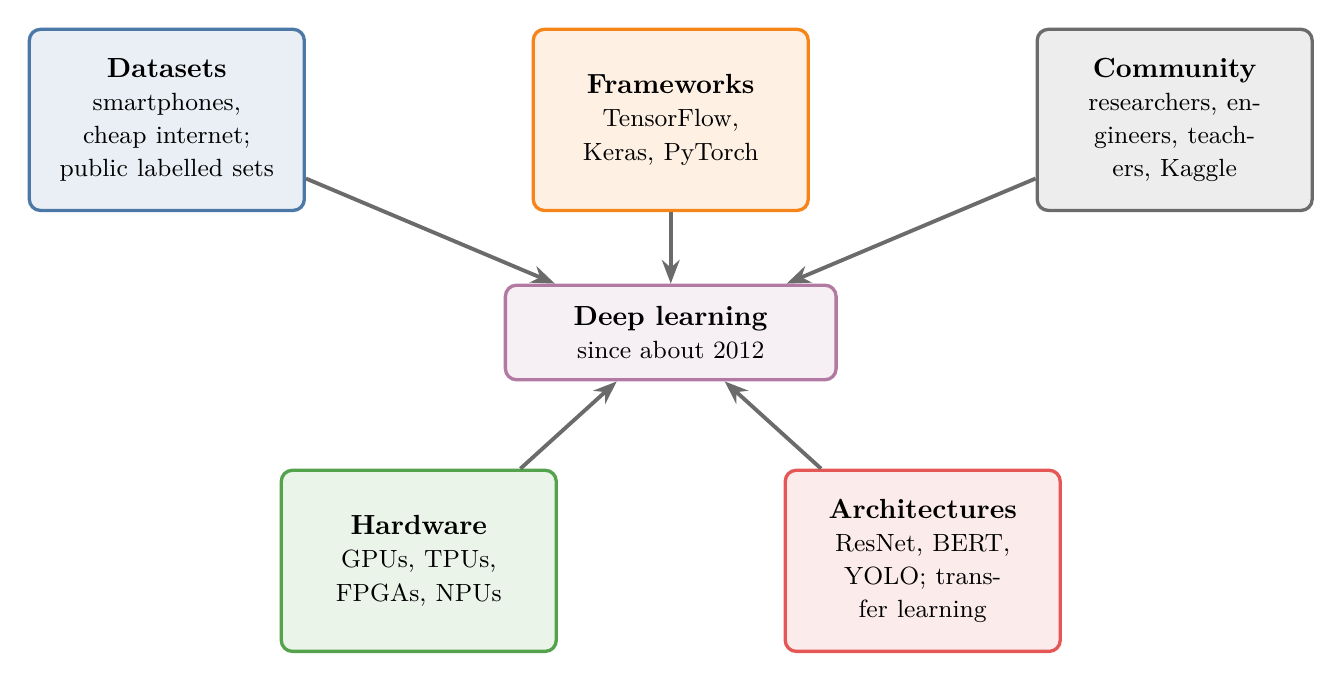
\begin{tikzpicture}[f/.style={box=#1, minimum width=3.2cm, text width=3.0cm, minimum height=2.3cm}]
  \node[box=cpurple, minimum width=4.2cm, minimum height=1.2cm] (dl) at (0,0) {\textbf{Deep learning}\\{\small since about 2012}};
  \node[f=cblue]   (d) at (-6.4,2.7) {\textbf{Datasets}\\{\small smartphones, cheap internet; public labelled sets}};
  \node[f=cgreen]  (h) at (-3.2,-2.9) {\textbf{Hardware}\\{\small GPUs, TPUs, FPGAs, NPUs}};
  \node[f=corange] (fw) at (0,2.7) {\textbf{Frameworks}\\{\small TensorFlow, Keras, PyTorch}};
  \node[f=cred]    (a) at (3.2,-2.9) {\textbf{Architectures}\\{\small ResNet, BERT, YOLO; transfer learning}};
  \node[f=cgrey]   (c) at (6.4,2.7) {\textbf{Community}\\{\small researchers, engineers, teachers, Kaggle}};
  \foreach \n in {d,h,fw,a,c} \draw[arrow] (\n) -- (dl);
\end{tikzpicture}
\end{document}
